\documentclass[14pt]{extbook}
\usepackage{multicol, enumerate, enumitem, hyperref, color, soul, setspace, parskip, fancyhdr} %General Packages
\usepackage{amssymb, amsthm, amsmath, bbm, latexsym, units, mathtools} %Math Packages
\everymath{\displaystyle} %All math in Display Style
% Packages with additional options
\usepackage[headsep=0.5cm,headheight=12pt, left=1 in,right= 1 in,top= 1 in,bottom= 1 in]{geometry}
\usepackage[usenames,dvipsnames]{xcolor}
\usepackage{dashrule}  % Package to use the command below to create lines between items
\newcommand{\litem}[1]{\item#1\hspace*{-1cm}\rule{\textwidth}{0.4pt}}
\pagestyle{fancy}
\lhead{Progress Quiz 3}
\chead{}
\rhead{Version B}
\lfoot{}
\cfoot{}
\rfoot{Fall 2020}
\begin{document}

\begin{enumerate}
\litem{
Solve the quadratic equation below. Then, choose the intervals that the solutions belong to, with $x_1 \leq x_2$ (if they exist).\[ 16x^{2} -14 x -7 = 0 \]\begin{enumerate}[label=\Alph*.]
\item \( x_1 \in [-0.86, 0.5] \text{ and } x_2 \in [1, 2.7] \)
\item \( x_1 \in [-6.04, -5.23] \text{ and } x_2 \in [19.2, 20.8] \)
\item \( x_1 \in [-25.42, -24.8] \text{ and } x_2 \in [25.6, 25.9] \)
\item \( x_1 \in [-1.32, -0.56] \text{ and } x_2 \in [0.2, 0.9] \)
\item \( \text{There are no Real solutions.} \)

\end{enumerate} }
\litem{
Solve the quadratic equation below. Then, choose the intervals that the solutions belong to, with $x_1 \leq x_2$ (if they exist).\[ -11x^{2} +10 x + 5 = 0 \]\begin{enumerate}[label=\Alph*.]
\item \( x_1 \in [-1.47, -0.73] \text{ and } x_2 \in [-0.5, 0.7] \)
\item \( x_1 \in [-14.46, -13.33] \text{ and } x_2 \in [3.2, 5.9] \)
\item \( x_1 \in [-17.7, -16.73] \text{ and } x_2 \in [17.2, 18.9] \)
\item \( x_1 \in [-0.57, -0.28] \text{ and } x_2 \in [1.1, 2.5] \)
\item \( \text{There are no Real solutions.} \)

\end{enumerate} }
\litem{
Factor the quadratic below. Then, choose the intervals that contain the constants in the form $(ax+b)(cx+d); b \leq d.$\[ 16x^{2} +32 x + 15 \]\begin{enumerate}[label=\Alph*.]
\item \( a \in [0.95, 1.81], \hspace*{5mm} b \in [7, 14], \hspace*{5mm} c \in [-0.68, 1.96], \text{ and } \hspace*{5mm} d \in [18, 21] \)
\item \( a \in [7.28, 8.66], \hspace*{5mm} b \in [2, 6], \hspace*{5mm} c \in [1.84, 2.65], \text{ and } \hspace*{5mm} d \in [1, 8] \)
\item \( a \in [3.94, 4.19], \hspace*{5mm} b \in [2, 6], \hspace*{5mm} c \in [2.76, 5.2], \text{ and } \hspace*{5mm} d \in [1, 8] \)
\item \( a \in [1.48, 2.23], \hspace*{5mm} b \in [2, 6], \hspace*{5mm} c \in [6.84, 9.53], \text{ and } \hspace*{5mm} d \in [1, 8] \)
\item \( \text{None of the above.} \)

\end{enumerate} }
\litem{
Graph the equation below.\[ f(x) = (x+4)^2 + 14 \]\begin{enumerate}[label=\Alph*.]
\begin{multicols}{2}\item 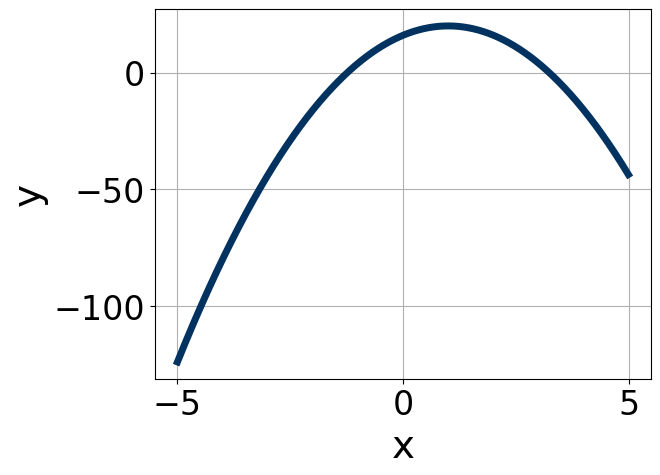
\includegraphics[width = 0.3\textwidth]{../Figures/quadraticEquationToGraphCopyAB.png}\item 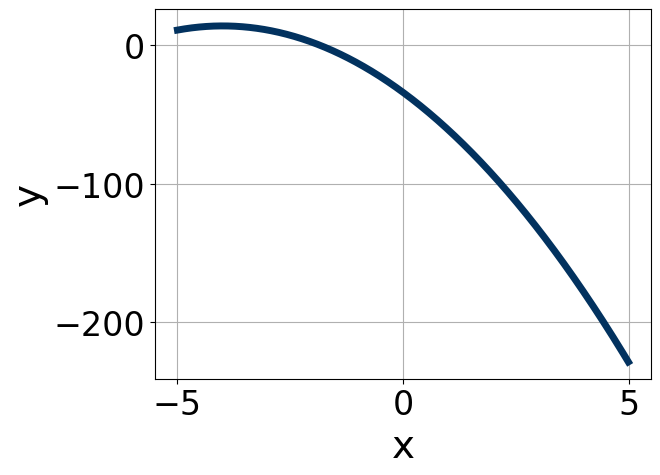
\includegraphics[width = 0.3\textwidth]{../Figures/quadraticEquationToGraphCopyBB.png}\item 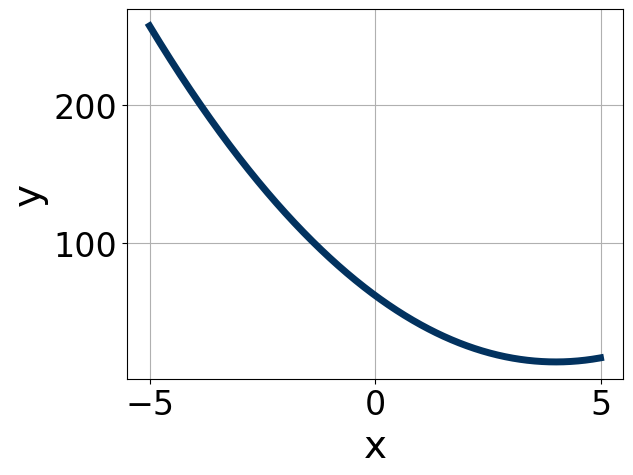
\includegraphics[width = 0.3\textwidth]{../Figures/quadraticEquationToGraphCopyCB.png}\item 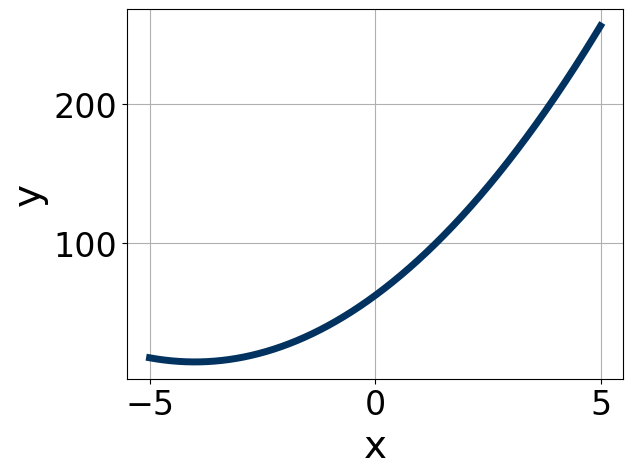
\includegraphics[width = 0.3\textwidth]{../Figures/quadraticEquationToGraphCopyDB.png}\end{multicols}\item None of the above.
\end{enumerate} }
\litem{
Factor the quadratic below. Then, choose the intervals that contain the constants in the form $(ax+b)(cx+d); b \leq d.$\[ 36x^{2} -60 x + 25 \]\begin{enumerate}[label=\Alph*.]
\item \( a \in [-3, 2.3], \hspace*{5mm} b \in [-30, -25], \hspace*{5mm} c \in [0.5, 1.8], \text{ and } \hspace*{5mm} d \in [-36, -29] \)
\item \( a \in [15.7, 20], \hspace*{5mm} b \in [-10, -1], \hspace*{5mm} c \in [1.8, 2.1], \text{ and } \hspace*{5mm} d \in [-5, -1] \)
\item \( a \in [4.5, 7.6], \hspace*{5mm} b \in [-10, -1], \hspace*{5mm} c \in [3.3, 8.4], \text{ and } \hspace*{5mm} d \in [-5, -1] \)
\item \( a \in [2.1, 3.2], \hspace*{5mm} b \in [-10, -1], \hspace*{5mm} c \in [10.9, 13.5], \text{ and } \hspace*{5mm} d \in [-5, -1] \)
\item \( \text{None of the above.} \)

\end{enumerate} }
\litem{
Solve the quadratic equation below. Then, choose the intervals that the solutions $x_1$ and $x_2$ belong to, with $x_1 \leq x_2$.\[ 6x^{2} -19 x -36 = 0 \]\begin{enumerate}[label=\Alph*.]
\item \( x_1 \in [-4, -3.66] \text{ and } x_2 \in [-3.2, 2.2] \)
\item \( x_1 \in [-0.76, 0.02] \text{ and } x_2 \in [12.1, 16.4] \)
\item \( x_1 \in [-8.24, -7.61] \text{ and } x_2 \in [23.2, 31.8] \)
\item \( x_1 \in [-1.81, -0.98] \text{ and } x_2 \in [4.4, 6.3] \)
\item \( x_1 \in [-2.95, -2.38] \text{ and } x_2 \in [1.9, 3.3] \)

\end{enumerate} }
\litem{
Graph the equation below.\[ f(x) = (x-2)^2 - 19 \]\begin{enumerate}[label=\Alph*.]
\begin{multicols}{2}\item 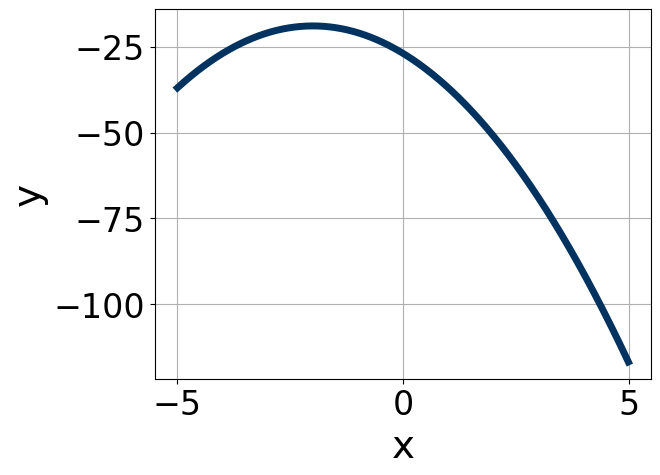
\includegraphics[width = 0.3\textwidth]{../Figures/quadraticEquationToGraphAB.png}\item 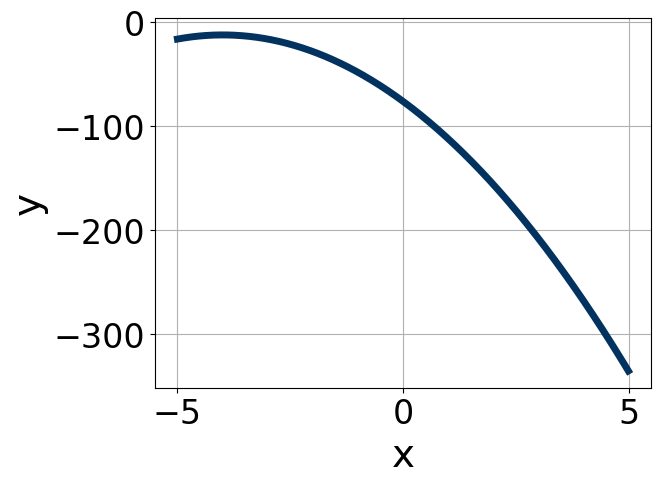
\includegraphics[width = 0.3\textwidth]{../Figures/quadraticEquationToGraphBB.png}\item 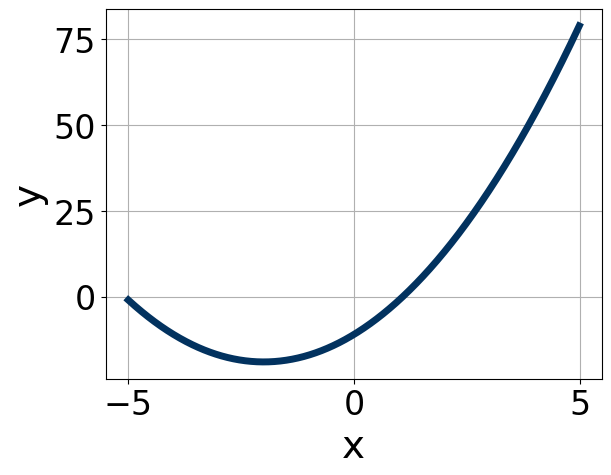
\includegraphics[width = 0.3\textwidth]{../Figures/quadraticEquationToGraphCB.png}\item 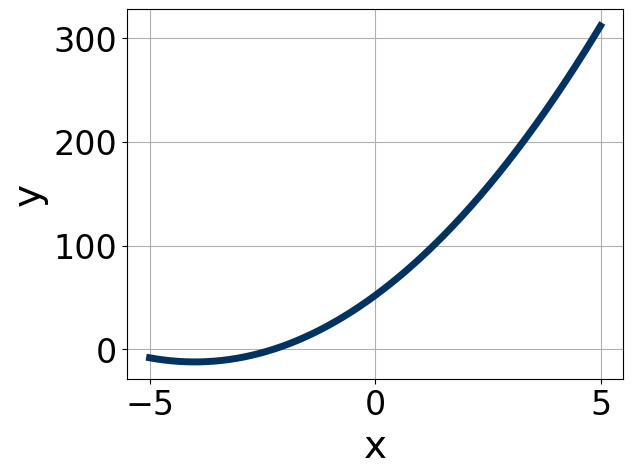
\includegraphics[width = 0.3\textwidth]{../Figures/quadraticEquationToGraphDB.png}\end{multicols}\item None of the above.
\end{enumerate} }
\litem{
Write the equation of the graph presented below in the form $f(x)=ax^2+bx+c$, assuming  $a=1$ or $a=-1$. Then, choose the intervals that $a, b,$ and $c$ belong to.
\begin{center}
    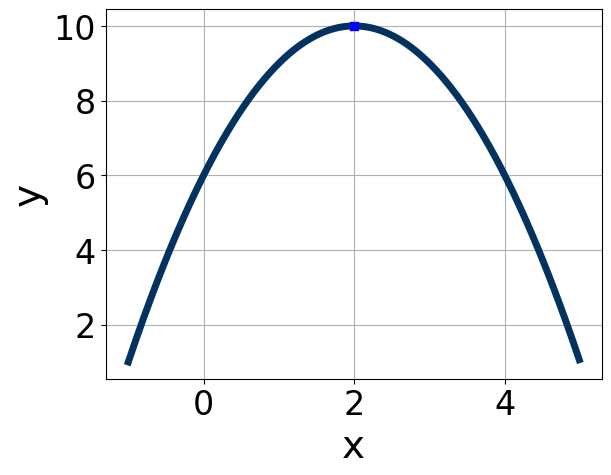
\includegraphics[width=0.5\textwidth]{../Figures/quadraticGraphToEquationCopyB.png}
\end{center}
\begin{enumerate}[label=\Alph*.]
\item \( a \in [-2, 0], \hspace*{5mm} b \in [-6, -3], \text{ and } \hspace*{5mm} c \in [-14, -11] \)
\item \( a \in [-2, 0], \hspace*{5mm} b \in [4, 6], \text{ and } \hspace*{5mm} c \in [6, 9] \)
\item \( a \in [0, 3], \hspace*{5mm} b \in [4, 6], \text{ and } \hspace*{5mm} c \in [13, 15] \)
\item \( a \in [0, 3], \hspace*{5mm} b \in [-6, -3], \text{ and } \hspace*{5mm} c \in [13, 15] \)
\item \( a \in [-2, 0], \hspace*{5mm} b \in [-6, -3], \text{ and } \hspace*{5mm} c \in [6, 9] \)

\end{enumerate} }
\litem{
Write the equation of the graph presented below in the form $f(x)=ax^2+bx+c$, assuming  $a=1$ or $a=-1$. Then, choose the intervals that $a, b,$ and $c$ belong to.
\begin{center}
    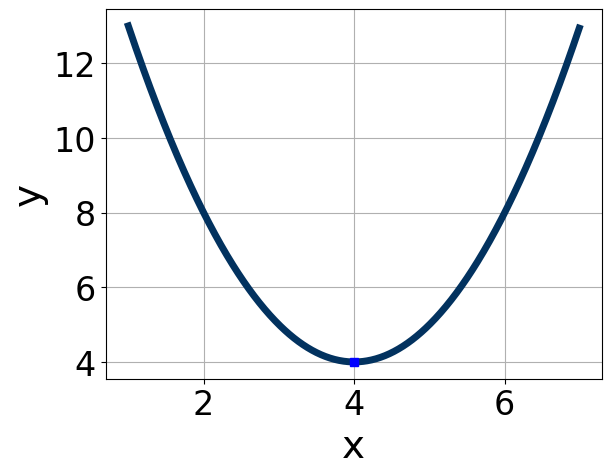
\includegraphics[width=0.5\textwidth]{../Figures/quadraticGraphToEquationB.png}
\end{center}
\begin{enumerate}[label=\Alph*.]
\item \( a \in [-2.2, -0.7], \hspace*{5mm} b \in [7, 11], \text{ and } \hspace*{5mm} c \in [-12, -11] \)
\item \( a \in [0.3, 2], \hspace*{5mm} b \in [-8, -5], \text{ and } \hspace*{5mm} c \in [20, 21] \)
\item \( a \in [0.3, 2], \hspace*{5mm} b \in [7, 11], \text{ and } \hspace*{5mm} c \in [10, 16] \)
\item \( a \in [0.3, 2], \hspace*{5mm} b \in [7, 11], \text{ and } \hspace*{5mm} c \in [20, 21] \)
\item \( a \in [-2.2, -0.7], \hspace*{5mm} b \in [-8, -5], \text{ and } \hspace*{5mm} c \in [-12, -11] \)

\end{enumerate} }
\litem{
Solve the quadratic equation below. Then, choose the intervals that the solutions $x_1$ and $x_2$ belong to, with $x_1 \leq x_2$.\[ 25x^{2} +60 x + 36 = 0 \]\begin{enumerate}[label=\Alph*.]
\item \( x_1 \in [-3.07, -1.95] \text{ and } x_2 \in [-0.66, -0.59] \)
\item \( x_1 \in [-3.81, -3.59] \text{ and } x_2 \in [-0.54, -0.28] \)
\item \( x_1 \in [-30.07, -29.89] \text{ and } x_2 \in [-30.1, -29.94] \)
\item \( x_1 \in [-6.3, -5.34] \text{ and } x_2 \in [-0.25, -0.07] \)
\item \( x_1 \in [-1.8, -0.79] \text{ and } x_2 \in [-1.3, -1.17] \)

\end{enumerate} }
\end{enumerate}

\end{document}